\documentclass[border=3mm]{standalone}
\usepackage{tikz}
\usetikzlibrary{arrows.meta,positioning,shapes.geometric,shapes.misc,fit,calc,backgrounds,decorations.pathreplacing,patterns}
\usepackage{amsmath,amssymb}

% ==============================================================================
% Color Palette: Rigorous, Accessible, Journal-Grade (Software: Practice and Exp)
% ==============================================================================
\definecolor{cSystem}{HTML}{1A5276}   % Slate Blue: Microservices & Telemetry
\definecolor{cChaos}{HTML}{D35400}    % Rich Amber/Orange: Faults & Threat Dynamics
\definecolor{cPolicy}{HTML}{5B2C6F}   % Deep Purple/Violet: DRL Controller & Policy
\definecolor{cMitig}{HTML}{196F3D}    % Emerald Green: Mitigation Queue & Actuators
\definecolor{cEval}{HTML}{21618C}     % Steel Blue: SRE Metrics & Resilience
\definecolor{cText}{HTML}{1C2833}     % Charcoal Text
\definecolor{cLightBg}{HTML}{FDFEFE}  % Crisp Background
\definecolor{cBorder}{HTML}{7F8C8D}   % Subtle Framing Gray

\begin{document}
\sffamily\footnotesize
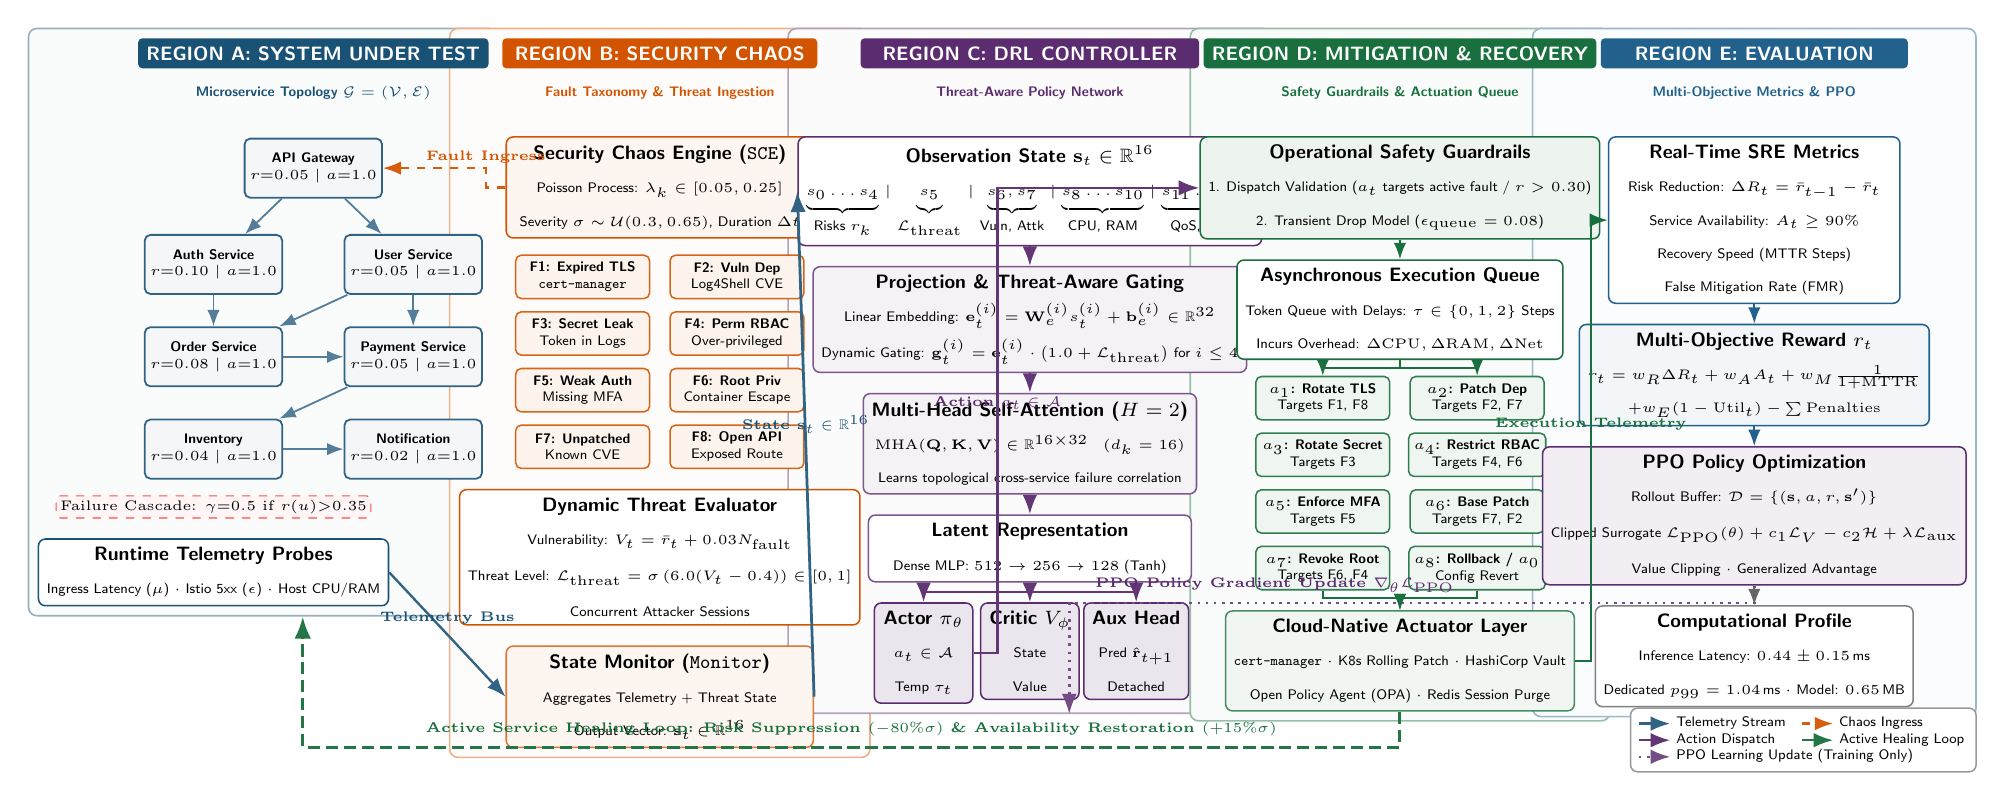
\begin{tikzpicture}[
    >=Latex,
    font=\sffamily,
    % Standard node types
    reglabel/.style={
        font=\sffamily\bfseries\scriptsize, text=white,
        rounded corners=1.5pt, inner sep=3pt, align=center
    },
    sublabel/.style={
        font=\sffamily\bfseries\tiny, align=center
    },
    card/.style={
        draw=black!70, line width=0.55pt, fill=white,
        rounded corners=2.5pt, inner sep=3pt, align=center
    },
    svcnode/.style={
        draw=cSystem!90, line width=0.65pt, fill=cSystem!5,
        rounded corners=2pt, inner sep=2pt, minimum width=15mm, minimum height=7.5mm,
        align=center, font=\sffamily\tiny
    },
    faultpill/.style={
        draw=cChaos!90, line width=0.55pt, fill=cChaos!7,
        rounded corners=2pt, inner sep=2pt, minimum width=17mm, minimum height=5.5mm,
        align=center, font=\sffamily\tiny
    },
    actionpill/.style={
        draw=cMitig!90, line width=0.55pt, fill=cMitig!7,
        rounded corners=2pt, inner sep=2pt, minimum width=17mm, minimum height=5.5mm,
        align=center, font=\sffamily\tiny
    },
    % Arrow connectors
    telemetryflow/.style={
        ->, line width=0.85pt, draw=cSystem!90
    },
    chaosflow/.style={
        ->, dashed, line width=0.8pt, draw=cChaos!95
    },
    controlflow/.style={
        ->, line width=0.9pt, draw=cPolicy!95
    },
    healloop/.style={
        ->, line width=1.1pt, draw=cMitig!95, dash pattern=on 4.5pt off 2pt
    },
    learnloop/.style={
        ->, line width=0.95pt, draw=cPolicy!85, dotted
    },
    normflow/.style={
        ->, line width=0.65pt, draw=black!75
    }
]

% ==============================================================================
% REGION A: SYSTEM UNDER TEST (MICROSERVICES & TELEMETRY)
% ==============================================================================
\node[reglabel, fill=cSystem, minimum width=38mm] (hdrA) at (0, 8.2) {REGION A: SYSTEM UNDER TEST};
\node[sublabel, text=cSystem, below=1mm of hdrA] (subA) {Microservice Topology $\mathcal{G} = (\mathcal{V}, \mathcal{E})$};

% 7 Service DAG Nodes
\node[svcnode, below=3.5mm of subA] (gw) {
    \textbf{API Gateway}\\
    $r{=}0.05 \mid a{=}1.0$
};
\node[svcnode, below left=4.5mm and -5mm of gw] (auth) {
    \textbf{Auth Service}\\
    $r{=}0.10 \mid a{=}1.0$
};
\node[svcnode, below right=4.5mm and -5mm of gw] (user) {
    \textbf{User Service}\\
    $r{=}0.05 \mid a{=}1.0$
};
\node[svcnode, below=4mm of auth] (order) {
    \textbf{Order Service}\\
    $r{=}0.08 \mid a{=}1.0$
};
\node[svcnode, below=4mm of user] (pay) {
    \textbf{Payment Service}\\
    $r{=}0.05 \mid a{=}1.0$
};
\node[svcnode, below=4mm of order] (inv) {
    \textbf{Inventory}\\
    $r{=}0.04 \mid a{=}1.0$
};
\node[svcnode, below=4mm of pay] (notif) {
    \textbf{Notification}\\
    $r{=}0.02 \mid a{=}1.0$
};

% Synchronous API Inter-Service Invocations
\draw[normflow, draw=cSystem!75] (gw) -- (auth);
\draw[normflow, draw=cSystem!75] (gw) -- (user);
\draw[normflow, draw=cSystem!75] (auth) -- (order);
\draw[normflow, draw=cSystem!75] (user) -- (order);
\draw[normflow, draw=cSystem!75] (user) -- (pay);
\draw[normflow, draw=cSystem!75] (order) -- (pay);
\draw[normflow, draw=cSystem!75] (pay) -- (inv);
\draw[normflow, draw=cSystem!75] (inv) -- (notif);

% Cascade Propagation Annotation
\node[draw=red!70, dashed, fill=red!4, rounded corners=1.5pt, inner sep=1.5pt, font=\tiny, below=2mm of inv] (cascade_lbl) {
    Failure Cascade: $\gamma{=}0.5$ if $r(u){>}0.35$
};

% Telemetry Probes Card
\node[card, draw=cSystem, fill=white, minimum width=38mm, below=2.5mm of cascade_lbl] (telemetry_probes) {
    \textbf{\scriptsize Runtime Telemetry Probes}\\
    \tiny Ingress Latency ($\mu$) $\cdot$ Istio 5xx ($\epsilon$) $\cdot$ Host CPU/RAM
};

% Region A Background Box
\begin{scope}[on background layer]
    \node[draw=cSystem!45, line width=0.6pt, fill=cSystem!2, rounded corners=3pt,
          fit=(hdrA) (subA) (gw) (notif) (cascade_lbl) (telemetry_probes)] (frameA) {};
\end{scope}

% ==============================================================================
% REGION B: SECURITY CHAOS & THREAT ASSESSMENT
% ==============================================================================
\node[reglabel, fill=cChaos, minimum width=40mm] (hdrB) at (4.4, 8.2) {REGION B: SECURITY CHAOS};
\node[sublabel, text=cChaos, below=1mm of hdrB] (subB) {Fault Taxonomy \& Threat Ingestion};

% Security Chaos Engine Core
\node[card, draw=cChaos, fill=cChaos!6, minimum width=39mm, below=3.5mm of subB] (sce_engine) {
    \textbf{\scriptsize Security Chaos Engine (\texttt{SCE})}\\
    \tiny Poisson Process: $\lambda_k \in [0.05, 0.25]$\\
    \tiny Severity $\sigma \sim \mathcal{U}(0.3, 0.65)$, Duration $\Delta t$
};

% 8 Standardized Faults
\node[faultpill, below=2mm of sce_engine, xshift=-9.8mm] (f_tls) {
    \textbf{F1: Expired TLS}\\
    \tiny \texttt{cert-manager}
};
\node[faultpill, below=2mm of sce_engine, xshift=9.8mm] (f_dep) {
    \textbf{F2: Vuln Dep}\\
    \tiny Log4Shell CVE
};
\node[faultpill, below=1.5mm of f_tls] (f_sec) {
    \textbf{F3: Secret Leak}\\
    \tiny Token in Logs
};
\node[faultpill, below=1.5mm of f_dep] (f_rbac) {
    \textbf{F4: Perm RBAC}\\
    \tiny Over-privileged
};
\node[faultpill, below=1.5mm of f_sec] (f_auth) {
    \textbf{F5: Weak Auth}\\
    \tiny Missing MFA
};
\node[faultpill, below=1.5mm of f_rbac] (f_priv) {
    \textbf{F6: Root Priv}\\
    \tiny Container Escape
};
\node[faultpill, below=1.5mm of f_auth] (f_patch) {
    \textbf{F7: Unpatched}\\
    \tiny Known CVE
};
\node[faultpill, below=1.5mm of f_priv] (f_api) {
    \textbf{F8: Open API}\\
    \tiny Exposed Route
};

% Dynamic Threat Evaluator
\node[card, draw=cChaos, fill=white, minimum width=39mm, below=2.5mm of f_patch, xshift=9.8mm] (threat_eval) {
    \textbf{\scriptsize Dynamic Threat Evaluator}\\
    \tiny Vulnerability: $V_t = \bar{r}_t + 0.03 N_{\mathrm{fault}}$\\[1pt]
    \tiny Threat Level: $\mathcal{L}_{\mathrm{threat}} = \sigma\left(6.0(V_t - 0.4)\right) \in [0, 1]$\\[1pt]
    \tiny Concurrent Attacker Sessions
};

% State Monitor Aggregator
\node[card, draw=cChaos!80, fill=cChaos!6, minimum width=39mm, below=2.5mm of threat_eval] (obs_aggregator) {
    \textbf{\scriptsize State Monitor (\texttt{Monitor})}\\
    \tiny Aggregates Telemetry + Threat State\\
    \tiny Output Vector: $\mathbf{s}_t \in \mathbb{R}^{16}$
};

% Region B Background Box
\begin{scope}[on background layer]
    \node[draw=cChaos!45, line width=0.6pt, fill=cChaos!2, rounded corners=3pt,
          fit=(hdrB) (subB) (sce_engine) (f_tls) (f_api) (threat_eval) (obs_aggregator)] (frameB) {};
\end{scope}

% ==============================================================================
% REGION C: THREAT-AWARE RL CONTROLLER
% ==============================================================================
\node[reglabel, fill=cPolicy, minimum width=43mm] (hdrC) at (9.1, 8.2) {REGION C: DRL CONTROLLER};
\node[sublabel, text=cPolicy, below=1mm of hdrC] (subC) {Threat-Aware Policy Network};

% State Vector Ingestion
\node[card, draw=cPolicy, fill=white, minimum width=41mm, below=3.5mm of subC] (ctrl_state) {
    \textbf{\scriptsize Observation State $\mathbf{s}_t \in \mathbb{R}^{16}$}\\
    \tiny $\underbrace{s_0 \dots s_4}_{\text{Risks } r_k} \mid \underbrace{s_5}_{\mathcal{L}_{\mathrm{threat}}} \mid \underbrace{s_6, s_7}_{\text{Vuln, Attk}} \mid \underbrace{s_8 \dots s_{10}}_{\text{CPU, RAM}} \mid \underbrace{s_{11} \dots s_{15}}_{\text{QoS, Status}}$
};

% Feature Projection & Gating Unit
\node[card, draw=cPolicy!80, fill=cPolicy!6, minimum width=41mm, below=2.5mm of ctrl_state] (ctrl_gating) {
    \textbf{\scriptsize Projection \& Threat-Aware Gating}\\
    \tiny Linear Embedding: $\mathbf{e}_t^{(i)} = \mathbf{W}_e^{(i)} s_t^{(i)} + \mathbf{b}_e^{(i)} \in \mathbb{R}^{32}$\\[1pt]
    \tiny Dynamic Gating: $\mathbf{g}_t^{(i)} = \mathbf{e}_t^{(i)} \cdot \left(1.0 + \mathcal{L}_{\mathrm{threat}}\right)$ for $i \le 4$
};

% Multi-Head Self-Attention
\node[card, draw=cPolicy!80, fill=cPolicy!6, minimum width=41mm, below=2.5mm of ctrl_gating] (ctrl_mhsa) {
    \textbf{\scriptsize Multi-Head Self-Attention ($H=2$)}\\
    \tiny $\mathrm{MHA}(\mathbf{Q}, \mathbf{K}, \mathbf{V}) \in \mathbb{R}^{16 \times 32} \quad (d_k=16)$\\
    \tiny Learns topological cross-service failure correlation
};

% Latent Dense Layers
\node[card, draw=cPolicy!80, fill=white, minimum width=41mm, below=2.5mm of ctrl_mhsa] (ctrl_dense) {
    \textbf{\scriptsize Latent Representation}\\
    \tiny Dense MLP: $512 \to 256 \to 128$ (Tanh)
};

% Decoupled Output Heads
\node[card, draw=cPolicy, fill=cPolicy!12, below=2.5mm of ctrl_dense, xshift=-13.5mm, minimum width=12.5mm] (h_actor) {
    \textbf{\scriptsize Actor $\pi_\theta$}\\
    \tiny $a_t \in \mathcal{A}$\\
    \tiny Temp $\tau_t$
};
\node[card, draw=cPolicy, fill=cPolicy!12, below=2.5mm of ctrl_dense, minimum width=12.5mm] (h_critic) {
    \textbf{\scriptsize Critic $V_\phi$}\\
    \tiny State\\
    \tiny Value
};
\node[card, draw=cPolicy, fill=cPolicy!12, below=2.5mm of ctrl_dense, xshift=13.5mm, minimum width=12.5mm] (h_aux) {
    \textbf{\scriptsize Aux Head}\\
    \tiny Pred $\hat{\mathbf{r}}_{t+1}$\\
    \tiny Detached
};

% Internal connections in Region C
\draw[controlflow] (ctrl_state) -- (ctrl_gating);
\draw[controlflow] (ctrl_gating) -- (ctrl_mhsa);
\draw[controlflow] (ctrl_mhsa) -- (ctrl_dense);
\draw[controlflow] (ctrl_dense.south) -- ++(0, -0.12) -| (h_actor.north);
\draw[controlflow] (ctrl_dense.south) -- (h_critic.north);
\draw[controlflow] (ctrl_dense.south) -- ++(0, -0.12) -| (h_aux.north);

% Region C Background Box
\begin{scope}[on background layer]
    \node[draw=cPolicy!45, line width=0.6pt, fill=cPolicy!2, rounded corners=3pt,
          fit=(hdrC) (subC) (ctrl_state) (ctrl_dense) (h_actor) (h_critic) (h_aux)] (frameC) {};
\end{scope}

% ==============================================================================
% REGION D: MITIGATION, QUEUE & RECOVERY
% ==============================================================================
\node[reglabel, fill=cMitig, minimum width=41mm] (hdrD) at (13.8, 8.2) {REGION D: MITIGATION \& RECOVERY};
\node[sublabel, text=cMitig, below=1mm of hdrD] (subD) {Safety Guardrails \& Actuation Queue};

% Operational Safety Guardrails
\node[card, draw=cMitig, fill=cMitig!8, minimum width=39mm, below=3.5mm of subD] (guard_shield) {
    \textbf{\scriptsize Operational Safety Guardrails}\\
    \tiny 1. Dispatch Validation ($a_t$ targets active fault / $r > 0.30$)\\
    \tiny 2. Transient Drop Model ($\epsilon_{\mathrm{queue}} = 0.08$)
};

% Asynchronous Execution Queue
\node[card, draw=cMitig, fill=white, minimum width=39mm, below=2.5mm of guard_shield] (async_queue) {
    \textbf{\scriptsize Asynchronous Execution Queue}\\
    \tiny Token Queue with Delays: $\tau \in \{0, 1, 2\}$ Steps\\
    \tiny Incurs Overhead: $\Delta\mathrm{CPU}, \Delta\mathrm{RAM}, \Delta\mathrm{Net}$
};

% 9 Supported Actions
\node[actionpill, below=2mm of async_queue, xshift=-9.8mm] (act_a1) {
    \textbf{$a_1$: Rotate TLS}\\
    \tiny Targets F1, F8
};
\node[actionpill, below=2mm of async_queue, xshift=9.8mm] (act_a2) {
    \textbf{$a_2$: Patch Dep}\\
    \tiny Targets F2, F7
};
\node[actionpill, below=1.5mm of act_a1] (act_a3) {
    \textbf{$a_3$: Rotate Secret}\\
    \tiny Targets F3
};
\node[actionpill, below=1.5mm of act_a2] (act_a4) {
    \textbf{$a_4$: Restrict RBAC}\\
    \tiny Targets F4, F6
};
\node[actionpill, below=1.5mm of act_a3] (act_a5) {
    \textbf{$a_5$: Enforce MFA}\\
    \tiny Targets F5
};
\node[actionpill, below=1.5mm of act_a4] (act_a6) {
    \textbf{$a_6$: Base Patch}\\
    \tiny Targets F7, F2
};
\node[actionpill, below=1.5mm of act_a5] (act_a7) {
    \textbf{$a_7$: Revoke Root}\\
    \tiny Targets F6, F4
};
\node[actionpill, below=1.5mm of act_a6] (act_a8) {
    \textbf{$a_8$: Rollback / $a_0$}\\
    \tiny Config Revert
};

% Actuator Layer
\node[card, draw=cMitig!80, fill=cMitig!6, minimum width=39mm, below=2.5mm of act_a7, xshift=9.8mm] (actuator_layer) {
    \textbf{\scriptsize Cloud-Native Actuator Layer}\\
    \tiny \texttt{cert-manager} $\cdot$ K8s Rolling Patch $\cdot$ HashiCorp Vault\\
    \tiny Open Policy Agent (OPA) $\cdot$ Redis Session Purge
};

% Internal connections in Region D
\draw[normflow, draw=cMitig] (guard_shield) -- (async_queue);
\draw[normflow, draw=cMitig] (async_queue.south) -- ++(0, -0.1) -| (act_a1.north);
\draw[normflow, draw=cMitig] (async_queue.south) -- ++(0, -0.1) -| (act_a2.north);
\draw[normflow, draw=cMitig] (act_a7.south) -- ++(0, -0.1) -| (actuator_layer.north);
\draw[normflow, draw=cMitig] (act_a8.south) -- ++(0, -0.1) -| (actuator_layer.north);

% Region D Background Box
\begin{scope}[on background layer]
    \node[draw=cMitig!45, line width=0.6pt, fill=cMitig!2, rounded corners=3pt,
          fit=(hdrD) (subD) (guard_shield) (async_queue) (act_a1) (act_a8) (actuator_layer)] (frameD) {};
\end{scope}

% ==============================================================================
% REGION E: EVALUATION & POLICY LEARNING FEEDBACK
% ==============================================================================
\node[reglabel, fill=cEval, minimum width=39mm] (hdrE) at (18.3, 8.2) {REGION E: EVALUATION};
\node[sublabel, text=cEval, below=1mm of hdrE] (subE) {Multi-Objective Metrics \& PPO};

% SRE Real-Time Metrics Card
\node[card, draw=cEval, fill=white, minimum width=37mm, below=3.5mm of subE] (sre_metrics) {
    \textbf{\scriptsize Real-Time SRE Metrics}\\
    \tiny Risk Reduction: $\Delta R_t = \bar{r}_{t-1} - \bar{r}_t$\\
    \tiny Service Availability: $A_t \ge 90\%$\\
    \tiny Recovery Speed (MTTR Steps)\\
    \tiny False Mitigation Rate (FMR)
};

% Multi-Objective Reward Card
\node[card, draw=cEval, fill=cEval!6, minimum width=37mm, below=2.5mm of sre_metrics] (eval_reward) {
    \textbf{\scriptsize Multi-Objective Reward $r_t$}\\
    \tiny $r_t = w_R \Delta R_t + w_A A_t + w_M \frac{1}{1 + \mathrm{MTTR}}$\\
    \tiny $+ w_E (1 - \mathrm{Util}_t) - \sum \mathrm{Penalties}$
};

% PPO Policy Optimization Loop
\node[card, draw=cPolicy, fill=cPolicy!8, minimum width=37mm, below=2.5mm of eval_reward] (eval_ppo) {
    \textbf{\scriptsize PPO Policy Optimization}\\
    \tiny Rollout Buffer: $\mathcal{D} = \{(\mathbf{s}, a, r, \mathbf{s}')\}$\\[1pt]
    \tiny Clipped Surrogate $\mathcal{L}_{\mathrm{PPO}}(\theta) + c_1 \mathcal{L}_V - c_2 \mathcal{H} + \lambda \mathcal{L}_{\mathrm{aux}}$\\[1pt]
    \tiny Value Clipping $\cdot$ Generalized Advantage
};

% Computational Profile Card
\node[card, draw=black!50, fill=white, minimum width=37mm, below=2.5mm of eval_ppo] (comp_profile) {
    \textbf{\scriptsize Computational Profile}\\
    \tiny Inference Latency: $0.44 \pm 0.15$\,ms\\
    \tiny Dedicated $p_{99} = 1.04$\,ms $\cdot$ Model: $0.65$\,MB
};

% Internal connections in Region E
\draw[normflow, draw=cEval] (sre_metrics) -- (eval_reward);
\draw[normflow, draw=cEval] (eval_reward) -- (eval_ppo);
\draw[normflow, draw=black!60] (eval_ppo) -- (comp_profile);

% Region E Background Box
\begin{scope}[on background layer]
    \node[draw=cEval!45, line width=0.6pt, fill=cEval!2, rounded corners=3pt,
          fit=(hdrE) (subE) (sre_metrics) (eval_reward) (eval_ppo) (comp_profile)] (frameE) {};
\end{scope}

% ==============================================================================
% INTER-REGION FLOW ARROWS & FEEDBACK LOOPS
% ==============================================================================

% 1. Chaos Ingress: SCE (Region B) -> Targeted Services in Region A
\draw[chaosflow] (sce_engine.west) -- ++(-0.25, 0) |- (gw.east)
    node[pos=0.35, above, font=\tiny\bfseries, text=cChaos] {Fault Ingress};

% 2. Telemetry Bus: Probes (Region A) -> State Monitor (Region B)
\draw[telemetryflow] (telemetry_probes.east) -- (obs_aggregator.west)
    node[pos=0.5, above, font=\tiny\bfseries, text=cSystem] {Telemetry Bus};

% 3. State Stream: State Monitor (Region B) -> State Vector (Region C)
\draw[telemetryflow, line width=1.0pt] (obs_aggregator.east) -- (ctrl_state.west)
    node[pos=0.5, above, font=\tiny\bfseries, text=cSystem] {State $\mathbf{s}_t \in \mathbb{R}^{16}$};

% 4. Action Dispatch: Actor Head (Region C) -> Safety Guardrails (Region D)
\draw[controlflow, line width=1.0pt] (h_actor.east) -- ++(0.3, 0) |- (guard_shield.west)
    node[pos=0.25, above, font=\tiny\bfseries, text=cPolicy] {Action $a_t \in \mathcal{A}$};

% 5. Actuation Telemetry: Actuators (Region D) -> Metrics (Region E)
\draw[normflow, draw=cMitig, line width=0.8pt] (actuator_layer.east) -- ++(0.2, 0) |- (sre_metrics.west)
    node[pos=0.25, above, font=\tiny\bfseries, text=cMitig] {Execution Telemetry};

% 6. Active Service Healing Loop: Actuators (Region D) -> Microservices (Region A)
% Routes cleanly beneath the diagram
\draw[healloop] (actuator_layer.south) -- ++(0, -0.45) -| ($(frameA.south) + (0.5, 0)$)
    node[pos=0.25, above, font=\tiny\bfseries, text=cMitig] {Active Service Healing Loop: Risk Suppression $(-80\%\sigma)$ \& Availability Restoration $(+15\%\sigma)$};

% 7. Closed-Loop Adaptation / Learning Feedback: PPO (Region E) -> Controller (Region C)
% Routes cleanly beneath Region E and D to Region C
\draw[learnloop] (eval_ppo.south) -- ++(0, -0.22) -| ($(frameC.south) + (0.5, 0)$)
    node[pos=0.35, above, font=\tiny\bfseries, text=cPolicy] {PPO Policy Gradient Update $\nabla_\theta \mathcal{L}_{\mathrm{PPO}}$};

% ==============================================================================
% COMPACT LEGEND (Bottom Right)
% ==============================================================================
\node[card, draw=black!40, fill=white, inner sep=2.5pt, anchor=south east] at ($(frameE.south east) + (0, -0.7)$) {
    \tiny
    \begin{tabular}{@{}l@{\quad}l@{}}
    \tikz[baseline=-0.5ex]\draw[telemetryflow, line width=0.9pt] (0,0) -- (4mm,0); Telemetry Stream &
    \tikz[baseline=-0.5ex]\draw[chaosflow, line width=0.8pt] (0,0) -- (4mm,0); Chaos Ingress \\
    \tikz[baseline=-0.5ex]\draw[controlflow, line width=0.9pt] (0,0) -- (4mm,0); Action Dispatch &
    \tikz[baseline=-0.5ex]\draw[healloop, line width=0.9pt] (0,0) -- (4mm,0); Active Healing Loop \\
    \multicolumn{2}{@{}l@{}}{\tikz[baseline=-0.5ex]\draw[learnloop, line width=0.9pt] (0,0) -- (4mm,0); PPO Learning Update (Training Only)}
    \end{tabular}
};

\end{tikzpicture}
\end{document}
